\documentclass[a4paper,12pt]{report}
\usepackage{times}
\usepackage{graphicx}
\usepackage[a4paper,
bindingoffset=0.2in,
left=1in,
right=.5in,
top=.7in,
bottom=.5in,
footskip=.25in]{geometry}
\usepackage{pdfpages}
\begin{document}
	\tableofcontents
	\listoffigures
	\newpage
\chapter{The Process and Stages of System Design}	
\section{Introduction}
The discussion is so far to a pivotal point in the system development life cycle. User requirements have been identified. Information has been gathered to verify the problem and evaluate the existing system. A feasibility analysis has been conducted to review alternative solutions and provide cost/benefit justification.  The culmination of the study is a proposal summarizing the finding and recommending a candidate system for the user.\\

If the figures and the reasoning behind the candidate system makes sense,management authorizes the proposed change. At this point in the system's life cycle, the design phase begins. The design phase is a solution, a “how to” approach,compared to analysis,a “what is”orientation. It translates the system requirements into ways of operationalizing them.\\
\textbf{The design phase is a translation from a user-oriented document to a document oriented to the programs or database personnel.} 
	\section{Logical and Physical Design}
	
	System design goes through two phases of development: logical and physical design. The design which shows the logical flow of a system and defines the boundaries of the system is known as \textbf{logical system design}. It describes the input,output,databases and procedures all in a format that meets the user requirements. The design covers the following: 
	\begin{enumerate}
		\item	Reviews the current physical system: its data flow , frequencies.
		\item 	Prepares output specification:it determines the format content and frequency of reports.
		\item 	Prepares input specification: format, content and most of the input functions
		\item 	Specifies the implementation plan.
		\item	Review benefits , costs, target dates and system constraints.
	\end{enumerate}
\begin{figure}[h]
	\centering
	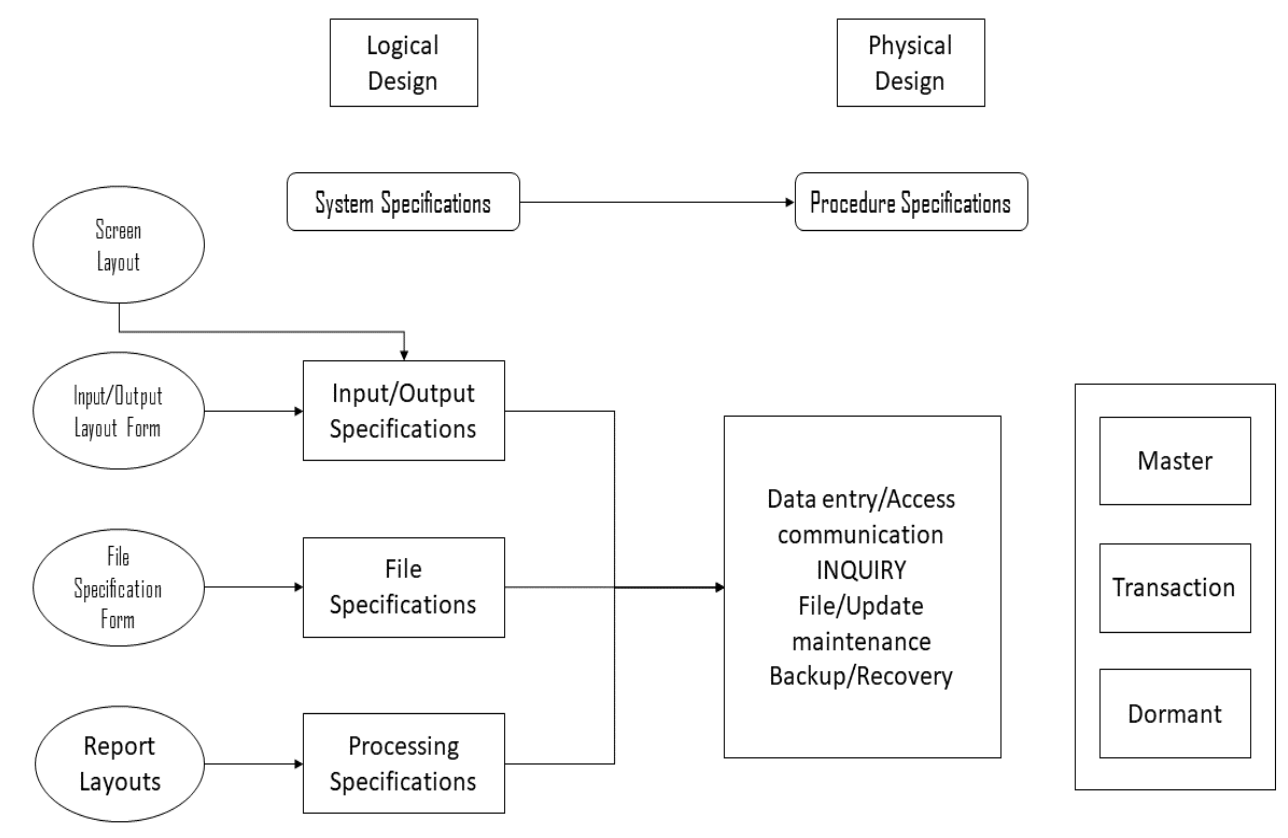
\includegraphics[width=0.7\linewidth]{9_1}
	\caption{system goes through Logical and Physical design}
	\label{fig:92}
\end{figure}
Physical design relates to the actual input and output processes of the system. It focuses on how data is entered into a system,verified, processed and displayed as output. It produces the working system by defining the design specification that specifies exactly what the candidate system does. It consist of following steps:	
	
	\begin{itemize}
		\item Specifying the input/output media, designing the database, and specifying    backup procedures.
		\item  Planning system implementation.
		\item  Devising a test and implementation plan, and specifying any new hardware         and software.
		\item  Updating costs, benefits, conversion dates, and system constraints.
		
	\end{itemize}
\section{Structured Design}

	Structured design is a data-flow-based methodology. The approach begins with a system specification that identifies input and output and describes the functional aspects of the system.  In structured designing, the system specifications act as a basis for graphically representing the flow of data and sequence of processes involved in a software development with the help of DFDs. After developing the DFDs for the software system, the next step is to develop the structure chart.
	
	
\begin{figure}[h]
	\centering
	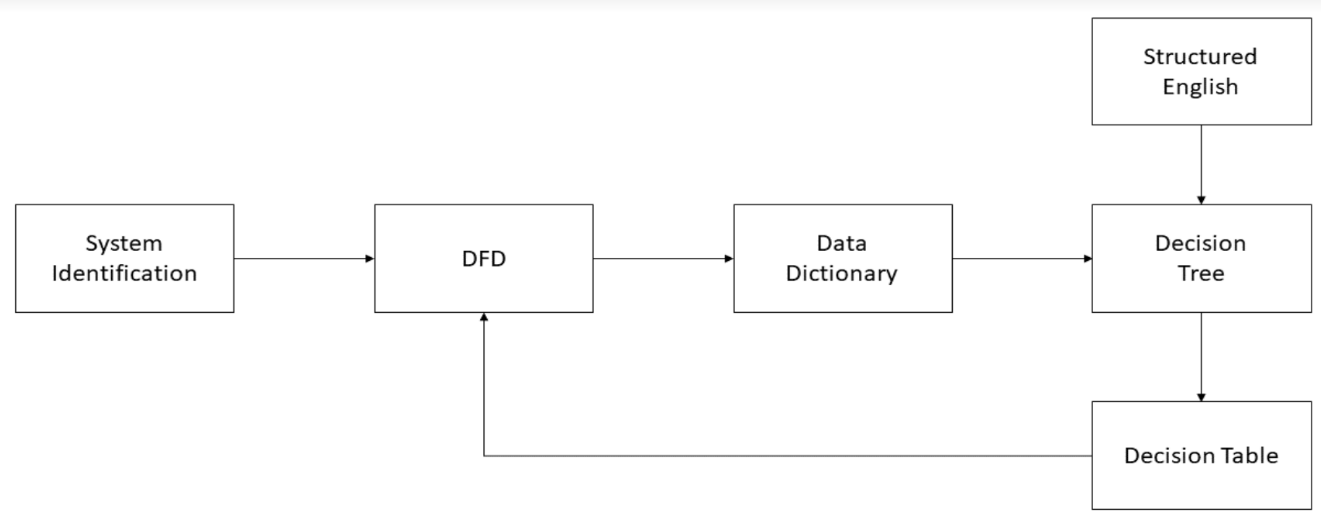
\includegraphics[width=0.7\linewidth]{9_2}
	\caption{Structured Design Method}
	\label{fig:92}
\end{figure}
\section{HIPO Diagram}
HIPO is a forms-driven technique in that standard forms are used to document the information. It consists of a hierarchy chart and an associated set of input/process/output charts. It captures the essence of top-down decomposition, it describes the data input and output from processes and defines the data flow composition. It was developed by IBM as a design aid and implementation technique.The overall design of the system is documented using HIPO charts or structure charts. The structure chart is similar in appearance to an organizational chart, but has been modified to show additional detail.
\begin{figure}
	\centering
	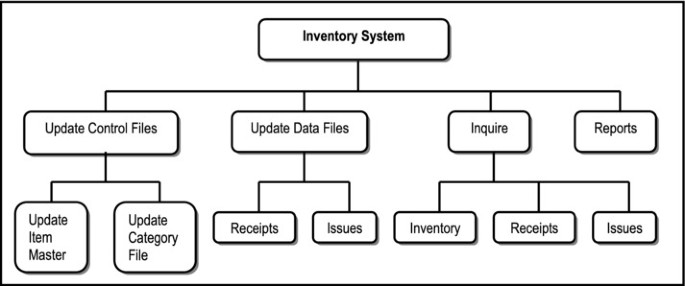
\includegraphics[width=0.7\linewidth]{9_3}
	\caption{HIPO Diagram for a project by NetaCode}
	\label{fig:93}
\end{figure}
\section{IPO Diagram}
An IPO (Input Process Output) Diagram is a very high level diagram used for system analysis that visually describes the business process with the description of each component in word. It shows a process key inputs and resulting output after a set of operations.
\begin{figure}
	\centering
	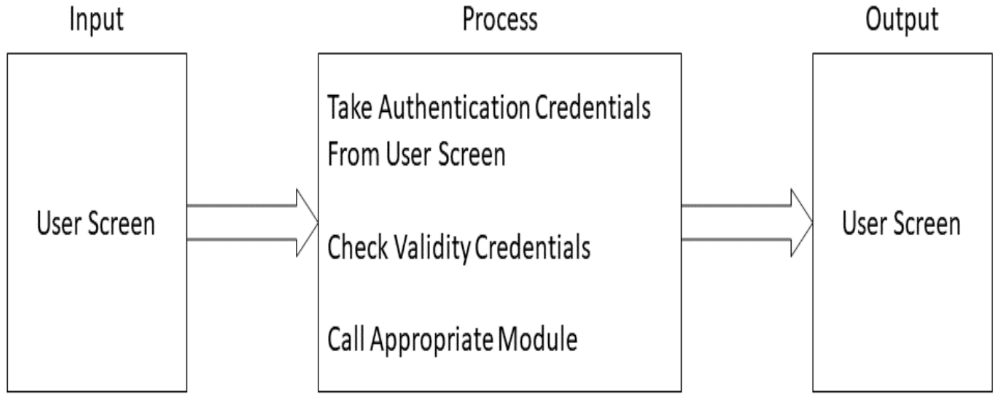
\includegraphics[width=0.7\linewidth]{9_4}
	\caption{IPO Diagram of NetaCode Implemented project}
	\label{fig:94}
\end{figure}
\paragraph{Summary}
System design is the phase that bridges the gap between problem domain and the existing system in a manageable way. This focuses on the solution domain,like how to implement. It is the phase where the SRS document is converted into a format that can be implemented and decides how the system will operate. In this phase the complex activity of system development is divided into several-sub-activities. Which coordinate with each other to achieve the main objective of system development.


	\end{document}